\subsection{Optimierter Common-Emitter-Verstärker} % (fold)
\label{sub:Optimierter_Common-Emitter-Verstärker}
\begin{frame}
    \frametitle{Optimierter Common-Emitter-Verstärker}
    \framesubtitle{}
    \begin{figure}[H]
    \begin{center}
            \includegraphics[scale=0.2]{./img/schaltungen/common_emitter_optimiert.png}
    \end{center}
    \end{figure}
\end{frame}
\begin{frame}
    \frametitle{Optimierter Common-Emitter-Verstärker}
    \framesubtitle{}
    \begin{columns}[c]
    \column{0.5\textwidth}
    \begin{figure}[H]
    \begin{center}
            \includegraphics[scale=0.15]{./img/schaltungen/common_emitter_optimiert.png}
    \end{center}
    \end{figure}
    \column{0.5\textwidth}
    \begin{block}{Funktionsweise}
        \begin{itemize}
            \item Stabilisierung des Transistors durch zusätzliche Bauelemente
            \item Kondensatoren wirken wie Hochpassfilter
            \item durch maximale Schaltfrequenz kann sich ein Tiefpass ergeben
        \end{itemize}     
    \end{block}
    \end{columns}
\end{frame}
\begin{frame}
    \frametitle{Optimierter Common-Emitter-Verstärker}
    \framesubtitle{Bodediagramme}
    \begin{figure}[H]
    \begin{center}
            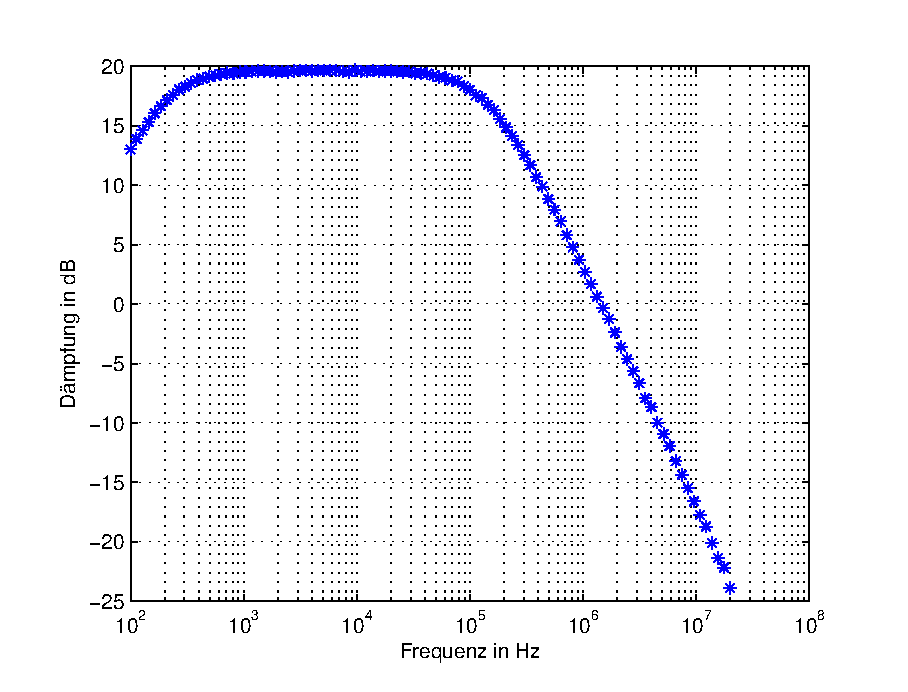
\includegraphics[scale=0.5]{./img/bode/Aufgabe_3_2_db.eps}
    \end{center}
    \end{figure}
\end{frame}
\begin{frame}
    \frametitle{Optimierter Common-Emitter-Verstärker}
    \framesubtitle{Bodediagramme}
    \begin{figure}[H]
    \begin{center}
            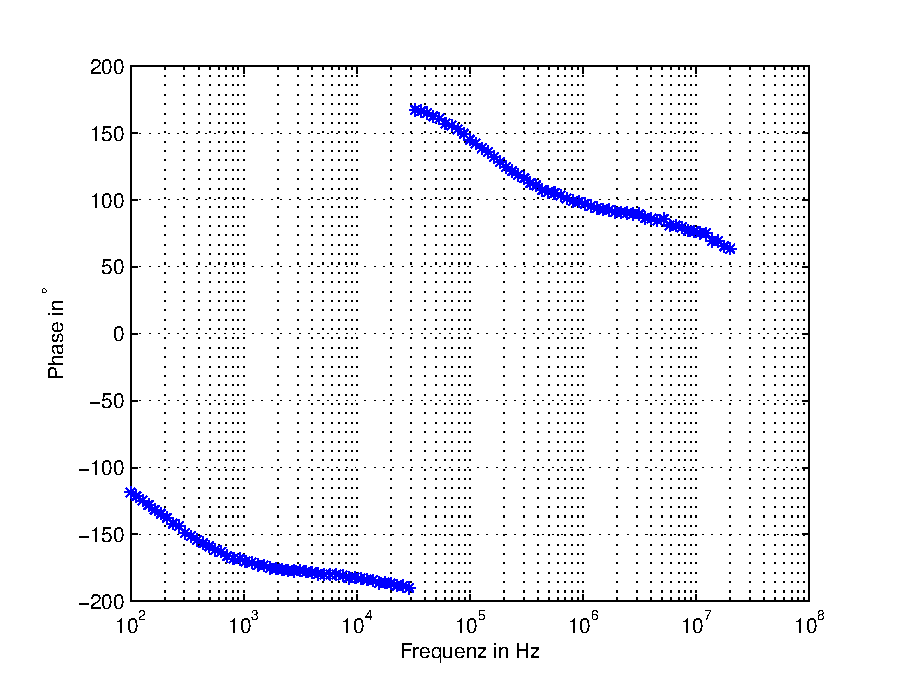
\includegraphics[scale=0.5]{./img/bode/Aufgabe_3_2_ph.eps}
    \end{center}
    \end{figure}
\end{frame}

% subsection Optimierter Common-Emitter-Verstärker (end)
